\documentclass[a4paper,12pt]{article}
\usepackage{extsizes}
\usepackage[utf8]{inputenc}
\usepackage[T1]{fontenc}
\usepackage[bulgarian]{babel}
\usepackage{amsmath}
\usepackage [full]{textcomp}
\usepackage{graphicx}
\DeclareGraphicsExtensions{.pdf,.png,.jpg}

%opening
\title{Курсов проект по
\\ \vspace{0.5cm} Въведение в системите основани на зная
\\ \vspace{2cm}\Large{Тема: Музикални инструменти}}
\author{Валентина Динкова, ф.н. 71112, 2 група}
\begin{document}

\maketitle

\newpage

\section{Кратко описание на йерархията}
Проектът се състои от 2 базови класа - един абстрактен - \textbf{\textit{Instrument}} и един конкретен -\textbf{ Musician}. Абстрактият клас \textbf{\textit{Instrument}} има 3 наследника - \textbf{Wind}, \textbf{String} и \textbf{Percussion}, които са конкретни класове:
\begin{itemize}
 \item \textbf{\textit{Instrument}}
  \begin{itemize}
   \item \textbf{Wind}
   \item \textbf{String}
   \item \textbf{Percussion}
  \end{itemize}
 \item \textbf{Musician}
\end{itemize}
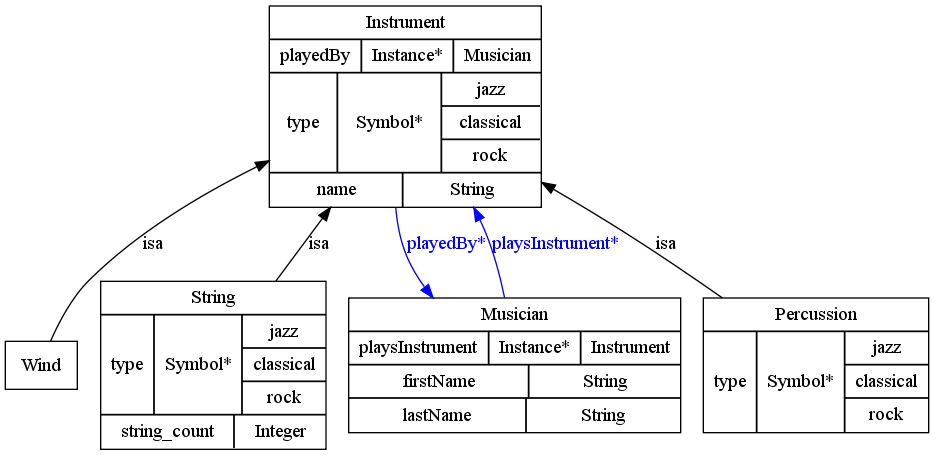
\includegraphics[width = 400px]{onto_graph.png}

\section{Кратко описание на дефинираните слотове}

\subsection{Слотове на класа \textbf{\textit{Instrument}}}

\begin{itemize}
 \item \textbf{name} - слот от тип \textit{string} с кардиналност \textit{required single};
\item \textbf{playedBy} - слот от тип \textit{instance of Musician} с кардиналност \textit{multiple}. Този слот е инверсен със слота \textit{playsInstrument} на класа \textbf{\textit{Musician}};
\item \textbf{type} - слот от тип \textit{symbol} с кардиналност \textit{required multiple}. Разрешените стойности за този слот са \textit{jazz}, \textit{classical} и \textit{rock};
\end{itemize}

Всички изброени по горе слотове имат дефиниционна област абстрактния клас \textbf{\textit{Instrument}}. Областта на действие на \textit{playedBy} е класа \textbf{Musician}.

\paragraph{String, Wind, Percussions:}
в тези класове слотовете, които са наследени от \textbf{\textit{Instrument}} имат дефиниционна област \textbf{\textit{Instrument}}. Новите слотове имат дефиниционна област съответния клас, към който принадлежат.

\subsection{Слотове на класа \textbf{Wind}}
Слотовете на класа \textbf{Wind} са наследени от абстрактния клас.


\subsection{Слотове на класа \textbf{String}}
Слотовете на класа \textbf{String} са наследени от абстрактния клас, като е добавен още един слот - \textit{string\_count} - от тип \textit{integer} и с кардиналност \textit{single}. Също така е предефиниран наследеният слот \textit{type} - зададена му е стойност по подразбиране \textit{rock}.

\subsection{Слотове на класа \textbf{Percussions}}
Слотовете на класа \textbf{Percussions} са наследени от абстрактния клас, като слота \textit{type} е предефиниран - зададена му е стойност по подразбиране \textit{rock}.

\subsection{Слотове на класа \textbf{Musician}}

\begin{itemize}
\item \textbf{firstName} - слот от тип \textit{string}  с кардиналност \textit{required single};
\item \textbf{lastName} - слот от тип \textit{string}  с кардиналност \textit{required single};
\item \textbf{playsInstrument} - слот от тип \textit{instance of Instrument} с кардиналност \textit{multiple}. Този слот е инверсен със слота \textit{playedBy} на класа \textbf{\textit{Instrument}};
\end{itemize}
Всички изброени по горе слотове имат дефиниционна област конкретния клас \textbf{Musician}. Областта на действие на \textit{playsInstrument} е класа \textbf{\textit{Instrument}}.

\section{Анкета}
Това, което ми хареса е идеята на CLIPS и Protege, но самата среда за разработка е доста нестабилна и и липсват някои удобства, които обикновено приемаме за нещо нормално, но в случая започнаха да ми се струват като лукс. Едно от тях е възможността за редактиране на ред в конзолата на CLIPS.

Курсът по въведение в системите основани на знания ми беше от полза и смятам че изнесеният материал както на семинарни упражнения, така и на лекции беше добре структуриран и с интересна тематика. Би било добре обаче да бъдат включени допълнително и практически упражнения в компютърна зала, като се обърне повече внимание на CLIPS.

\end{document}
